% ----------------------------------------------------------
\chapter{Testes}\label{cap:testes}
% ----------------------------------------------------------

Este capítulo descreve os procedimentos de teste adotados para avaliar a arquitetura proposta, abrangendo ambiente, cenários, métricas, coleta e análise dos dados.

% ----------------------------------------------------------
\section{Contextualização do Problema}
% ----------------------------------------------------------

Para avaliar a arquitetura proposta, foi adotado um cenário inspirado em aplicações de cidades inteligentes, com foco na gestão de recursos de água e energia. Nesse contexto, foram considerados medidores inteligentes que enviam dados de consumo para uma camada de névoa, onde ocorre o pré-processamento das informações antes de seu encaminhamento à nuvem.

Os dados utilizados para simulação foram obtidos a partir de conjuntos públicos, sendo um relacionado ao consumo residencial de energia elétrica \cite{uci_energy} e outro referente a medições de consumo de água \cite{greek_water}.

Antes da utilização nos testes, ambos os conjuntos de dados passaram por um processo de pré-processamento que incluiu a remoção de informações não essenciais e a agregação das medições em intervalos horários. Esse tratamento visou manter apenas os elementos relevantes para simular a operação contínua dos dispositivos, aproximando o comportamento dos dados ao fluxo esperado em um ambiente real de monitoramento urbano.

% ----------------------------------------------------------
\section{Ambiente de Testes}
% ----------------------------------------------------------

O ambiente de testes foi configurado para representar um cenário de cidade inteligente, no qual cada domínio de névoa corresponde a um bairro distinto. Cada névoa pode conter um nó primário, um nó agregador e um número variável de nós de névoa e dispositivos, de acordo com a demanda e o tipo de aplicação simulada.

A implantação e o gerenciamento desses componentes foram realizados por meio de uma interface web desenvolvida para este trabalho, que interage diretamente com o Docker para criar e controlar as instâncias. Essa interface permite selecionar o bairro (névoa) no qual os componentes serão implantados, definir o tipo de contêiner e a quantidade de instâncias, além de oferecer controle individual ou em grupo para iniciar, pausar, parar e visualizar logs.

A Figura~\ref{fig:container_manager} apresenta a tela de gerenciamento de contêineres para o bairro Canasvieiras. Nela, observa-se a criação de um nó de névoa e de um medidor de energia, ambos em execução. O painel agrupa as instâncias por tipo de componente, permitindo visualizar rapidamente seu estado e realizar ações sobre cada grupo ou instância individual.

\begin{figure}[htb]
    \caption{\label{fig:container_manager}Interface para gerenciamento de contêineres no ambiente de testes.}
    \begin{center}
        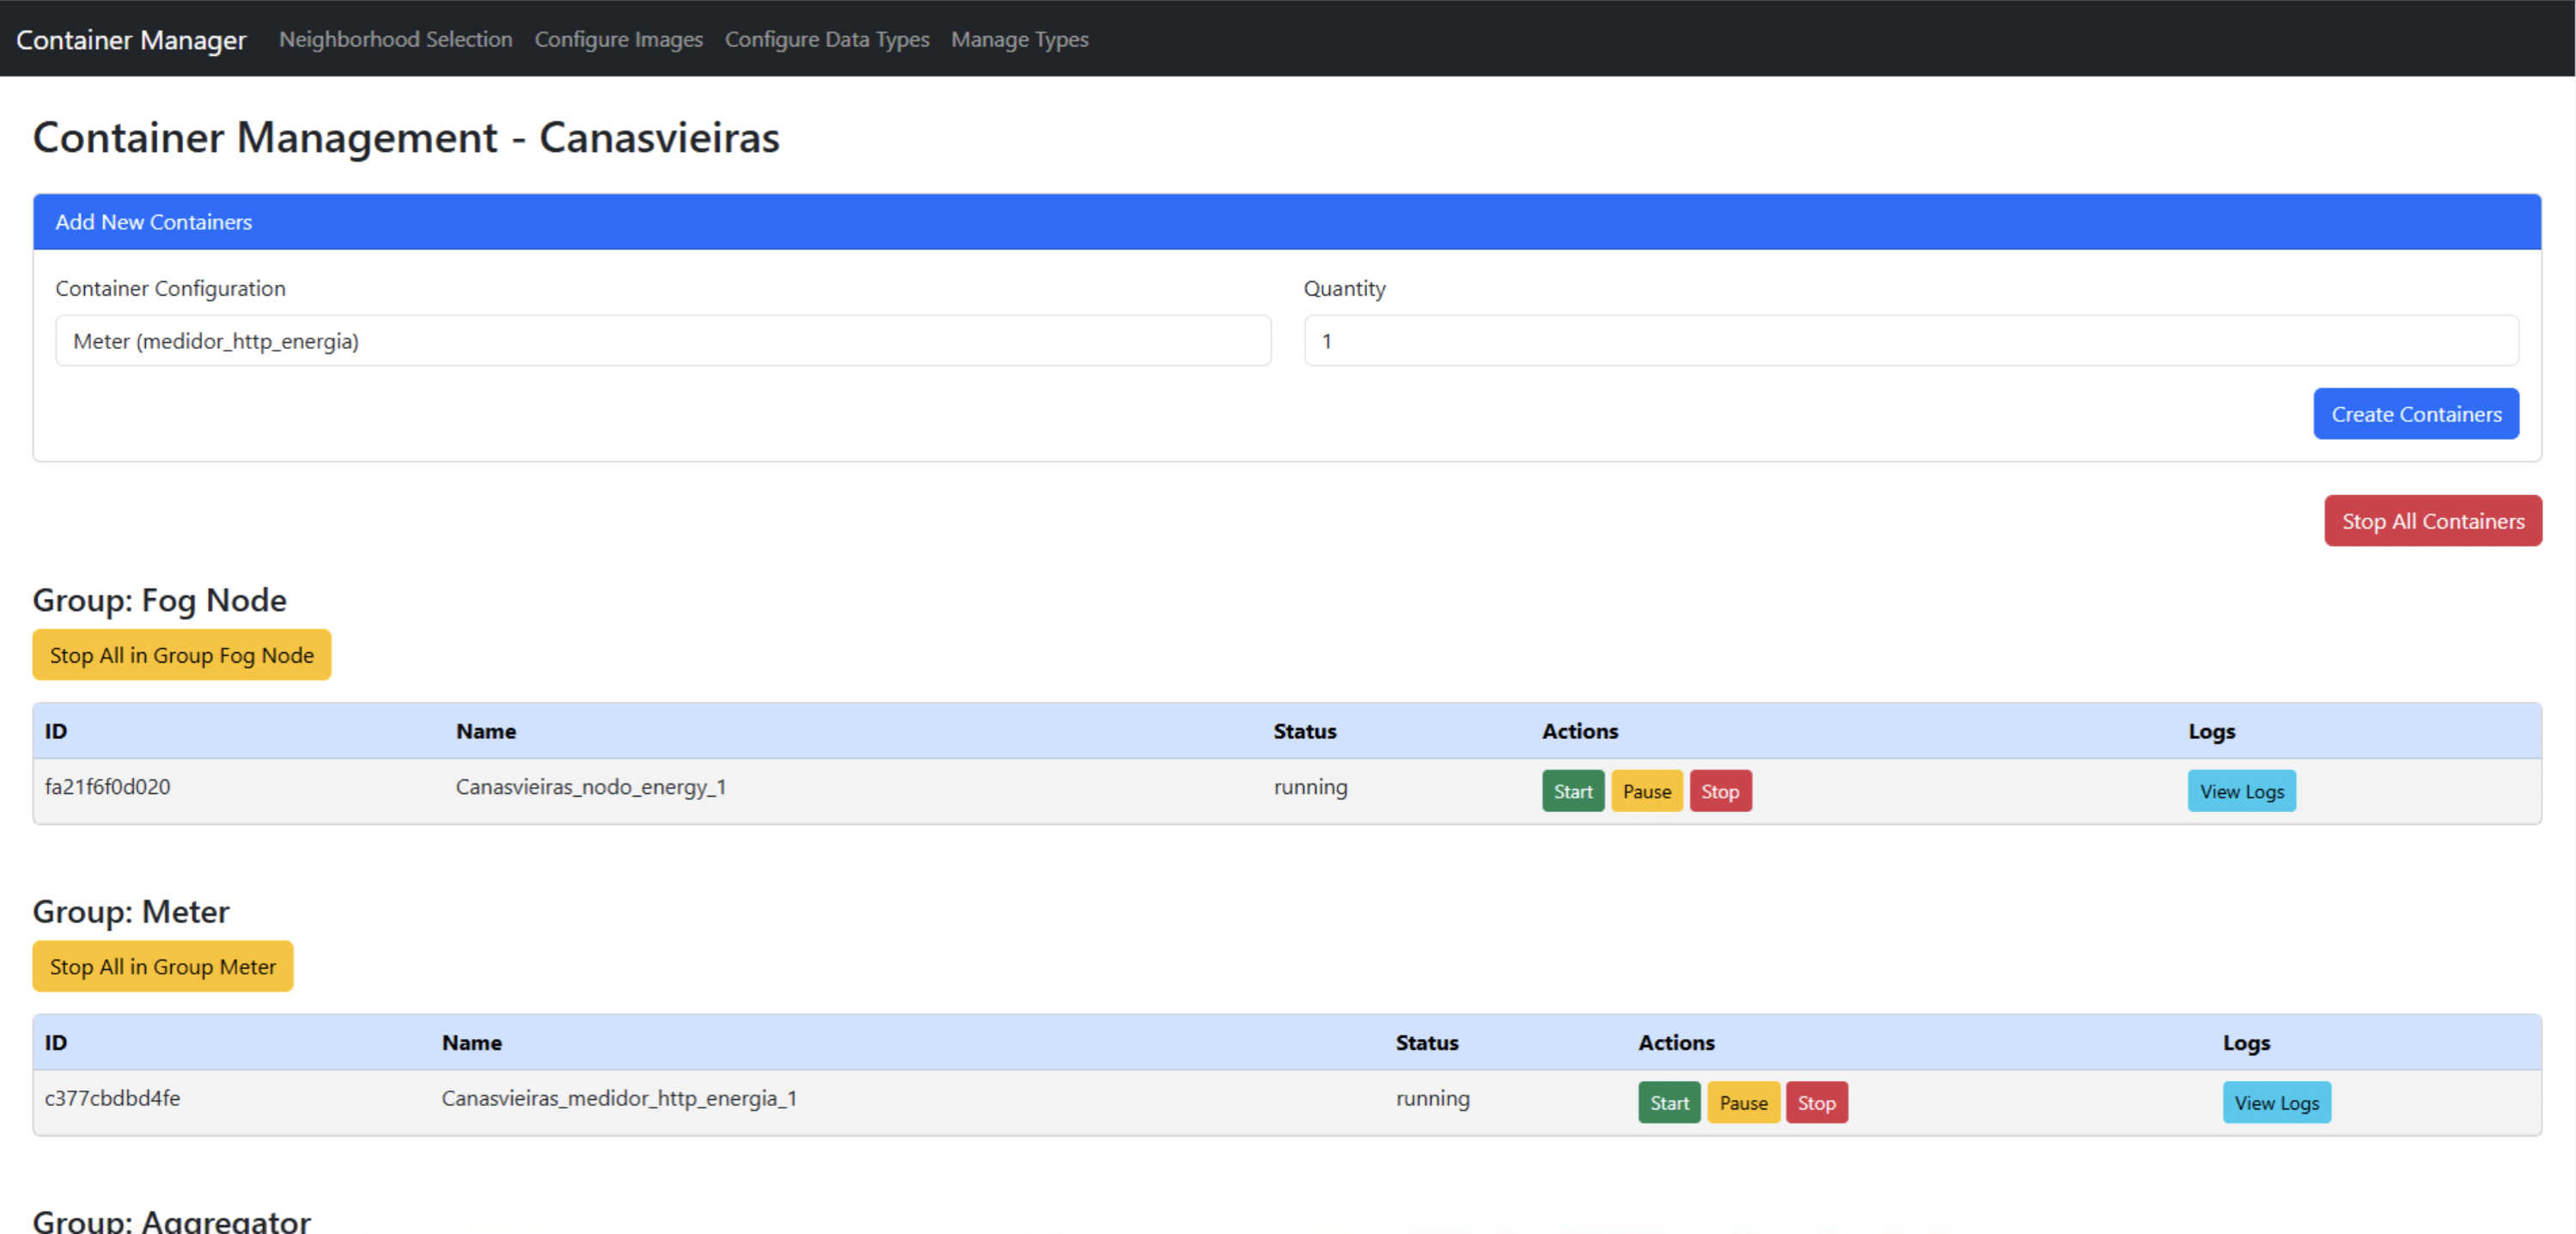
\includegraphics[width=1\linewidth]{images/container_manager.png}
    \end{center}
    \fonte{Do autor.}
\end{figure}

% ----------------------------------------------------------
\subsection{Tecnologias e Ambiente Físico}
% ----------------------------------------------------------

No ambiente de testes, todos os componentes da arquitetura foram implementados em \textit{Python}, com exceção do medidor compatível com o protocolo \textit{CoAP}, que foi desenvolvido em \textit{Node.js} devido à disponibilidade de bibliotecas específicas e otimização do fluxo de comunicação nesse protocolo.

Os experimentos foram executados em uma única máquina física, utilizada para hospedar os contêineres Docker que compõem cada instância de nó e dispositivo. A Tabela~\ref{tab:especificacoes_maquina} apresenta as especificações do equipamento utilizado.

\begin{table}[htb]
    \caption{\label{tab:especificacoes_maquina}Especificações da máquina utilizada nos testes.}
    \centering
    \begin{tabular}{ll}
        \hline
            \textbf{Componente} & \textbf{Especificação} \\
        \hline
            Processador & Intel Core i7-7700K @ 4.20GHz \\
            Memória RAM & 32 GB DDR4 \\
            Armazenamento & SSD 2 TB \\
            Sistema Operacional & Windows 11 \\
            Docker & v4.38.0 \\
        \hline
    \end{tabular}
    \fonte{Do autor.}
\end{table}

% ----------------------------------------------------------
\section{Protocolos}
% ----------------------------------------------------------

No ambiente de testes, o nó primário é responsável por receber dados utilizando diferentes protocolos, incluindo \textit{CoAP}, \textit{MQTT} e \textit{HTTP}. Independentemente do protocolo de origem, as mensagens são convertidas para \textit{HTTP} antes de serem encaminhadas aos nós de névoa, de forma a padronizar o tráfego interno.

Dentro de um nó de névoa, a comunicação entre a camada de protocolos e a camada de processamento ocorre por meio de \textit{WebSocket}, mantendo a conexão aberta para evitar o custo de abertura e fechamento contínuo de conexões. Essa abordagem reduz a sobrecarga e melhora o tempo de resposta.

A partir do nó de névoa, os dados já passam a ser organizados em estrutura \textit{CSV}, formada a partir das informações recebidas em \textit{JSON}. Essa etapa permite preparar os dados para compatibilidade com o formato aceito pela nuvem. A transmissão do nó de névoa para o nó agregador é realizada via \textit{SFTP}.

No nó agregador, os arquivos \textit{CSV} recebidos de diferentes nós de névoa são consolidados em um único arquivo antes de serem enviados para a camada de nuvem, também via \textit{SFTP}, para a zona de entrada (\textit{landing zone}) do \textit{HPCC Systems}.

% ----------------------------------------------------------
\section{Distribuição entre Névoas e Balanceamento de Carga}
% ----------------------------------------------------------

Nos experimentos, os \(120\) dispositivos foram distribuídos entre dois domínios de névoa distintos, representando diferentes regiões no cenário de cidade inteligente.  
A distribuição inicial foi a seguinte:

\begin{itemize}
    \item \textbf{Névoa A}: \(70\) dispositivos  
    (\(12\) medidores de energia via \textit{HTTP}, \(12\) via \textit{CoAP}, \(12\) via \textit{MQTT}, \(12\) medidores de água via \textit{HTTP}, \(12\) via \textit{CoAP}, \(10\) via \textit{MQTT}).
    \item \textbf{Névoa B}: \(50\) dispositivos  
    (\(8\) medidores de energia via \textit{HTTP}, \(8\) via \textit{CoAP}, \(8\) via \textit{MQTT}, \(8\) medidores de água via \textit{HTTP}, \(8\) via \textit{CoAP}, \(10\) via \textit{MQTT}).
\end{itemize}

Essa distribuição propositalmente desigual permitiu avaliar o comportamento do sistema sob condições de carga diferentes entre os domínios.  
Quando uma das névoas atingiu maior taxa de utilização, o mecanismo de balanceamento foi acionado: o nó primário da névoa mais carregada redirecionou parte das requisições para a outra, realizando a conversão para \textit{HTTP} antes do envio, independentemente do protocolo de origem (\textit{HTTP}, \textit{CoAP} ou \textit{MQTT}).

Nos testes, foram simulados dois dias de operação (\(48\ \text{horas}\)), com cada dispositivo enviando leituras periódicas agregadas em janela horária de consumo.

No nó agregador, as medições de cada domínio de névoa foram consolidadas em um único arquivo por dia e transmitidas para o \textit{HPCC Systems} ao final de cada dia, sem que nenhum contêiner apresentasse falhas durante a execução.

% ----------------------------------------------------------
\section{GraphQL}
% ----------------------------------------------------------

Nos nós de névoa, a comunicação entre a camada de serviços e a camada de processamento é realizada utilizando \textit{GraphQL} como linguagem de consulta de dados. Essa abordagem permite que a aplicação especifique exatamente quais campos e registros deseja receber, evitando transferências desnecessárias e reduzindo a sobrecarga de processamento.  

O \textit{GraphQL} possibilita ainda a consulta a múltiplas fontes de dados de forma unificada, agregando resultados distintos em uma única resposta. Nos testes realizados, o armazenamento local temporário nos nós de névoa foi implementado com \textit{MongoDB}, escolhido por sua flexibilidade para lidar com dados em formato \texttt{JSON} e pela capacidade de inserir registros heterogêneos sem a exigência de um esquema fixo.  

Com essa integração, a camada de serviços consegue solicitar à camada de processamento apenas as informações estritamente necessárias para o pré-processamento, recebendo uma resposta já filtrada e adaptada ao contexto da aplicação. Isso mantém a arquitetura modular, otimiza o fluxo de dados interno e garante maior agilidade na execução das tarefas.

% ----------------------------------------------------------
\section{HPCC Systems na Camada de Nuvem}
% ----------------------------------------------------------

Na fase de testes, os dados consolidados pelos nós agregadores foram enviados para a camada de nuvem, implementada com o \textit{HPCC Systems}. Os arquivos recebidos, no formato \texttt{.csv} suportado pela plataforma, resultam da união dos pré-processamentos realizados nos diferentes nós de névoa, reunidos pelo nó agregador antes da transmissão.  

Esses arquivos foram disponibilizados na zona de entrada da plataforma (\textit{landing zone}), onde ficaram prontos para processamento e consultas.  

A Figura~\ref{fig:hpcc_landing_zone} apresenta o ambiente \textit{ECL Watch}, mostrando os arquivos agregados de consumo de energia, já no formato consolidado por data, prontos para serem tratados ou analisados conforme as necessidades da aplicação.

\begin{figure}[htb]
    \caption{\label{fig:hpcc_landing_zone}Arquivos consolidados na \textit{landing zone} do HPCC Systems.}
    \begin{center}
        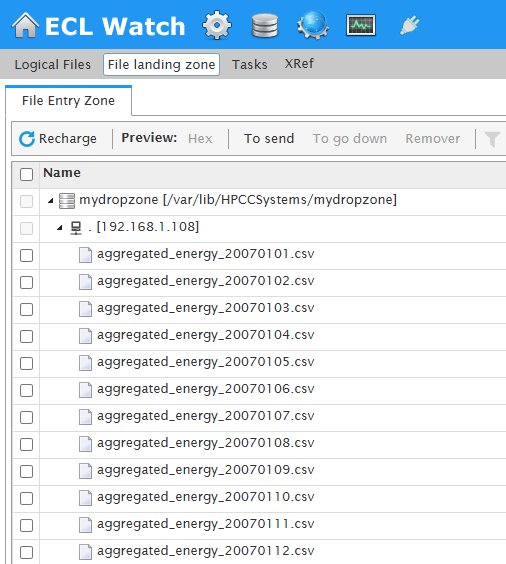
\includegraphics[width=0.7\linewidth]{images/hpcc_landing_zone.png}
    \end{center}
    \fonte{Do autor.}
\end{figure}
